% Chapter 3

\chapter{The Large Hadron Collider} % Chapter title

\label{ch:lhc} % For referencing the chapter elsewhere, use \autoref{ch:mathtest}

%----------------------------------------------------------------------------------------

The \ac{LHC} is unique in the world, producing proton-proton collisions at energies an order of magnitude higher than any accelerator before \cite{1748-0221-3-08-S08001}. It provides unique environments at its collision points where massive, unstable particles can exist for an instant, then decay to the ordinary material of the universe. It is the goal of the ATLAS experiment to identify these short-lived particles, but \ac{LHC}'s work of producing them is equally complex. 

The \ac{LHC} sits in a 26.7 km circular tunnel that straddles the French-Swiss border outside of Geneva, originally built in 1989 for the \ac{LEP} collider \cite{lep_tdr}. In the \ac{LHC}, two beams of protons are accelerated to 6.5 \tev, then focused and collided at four points around the ring, which can be seen in \autoref{fig:lhc_map}. These points are each encased by particle detectors, which can examine the outputs of the collisions, and have different strengths and goals. The two multipurpose detectors are ATLAS and \ac{CMS}, which have very complex detectors aimed and measuring as many \ac{SM} particles as possible and discovering new processes \cite{PERF-2007-01, 1748-0221-3-08-S08004}. \ac{LHCb} examines processes related to the $b$ quark \cite{1748-0221-3-08-S08005}. Meanwhile, \ac{ALICE} focuses on special runs of the \ac{LHC} which collide lead ions instead of protons, and seeks to understand the high energy densities resulting from the collisions of such massive, complex particles \cite{1748-0221-3-08-S08002}. 

\begin{centering}
\begin{figure}[!hbt]
\myfloatalign
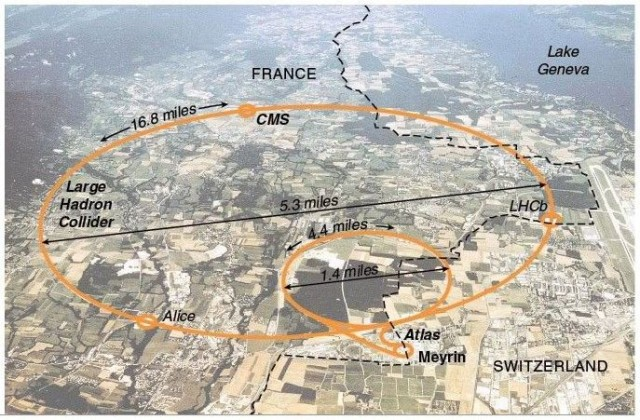
\includegraphics[width=.90\linewidth]{figures/lhc/lhc-5-640x420.jpg}
\caption{The \ac{LHC} main collider ring and pre-accelerator \ac{SPS} overlaid on a map of Switzerland and France, with the four main \ac{LHC} experiments identified.}
\label{fig:lhc_map}
\end{figure}
\end{centering}

%----------------------------------------------------------------------------------------

\section{The Injector Complex}

The goal of the \ac{LHC} is to provide high luminosity proton-proton collisions at 13 \tev. To achieve this, it must be capable of rapidly accelerating large numbers of protons and holding them at a constant energy, and organizing them into bunches which can be focused and collided at precise points and times. To do this, a complex system of pre-accelerators is required, as well as a precisely engineered sytem of magnets within the \ac{LHC}. The full system of pre-accelerators is shown in \autoref{fig:preacc}.

\begin{centering}
\begin{figure}[!hbt]
\myfloatalign
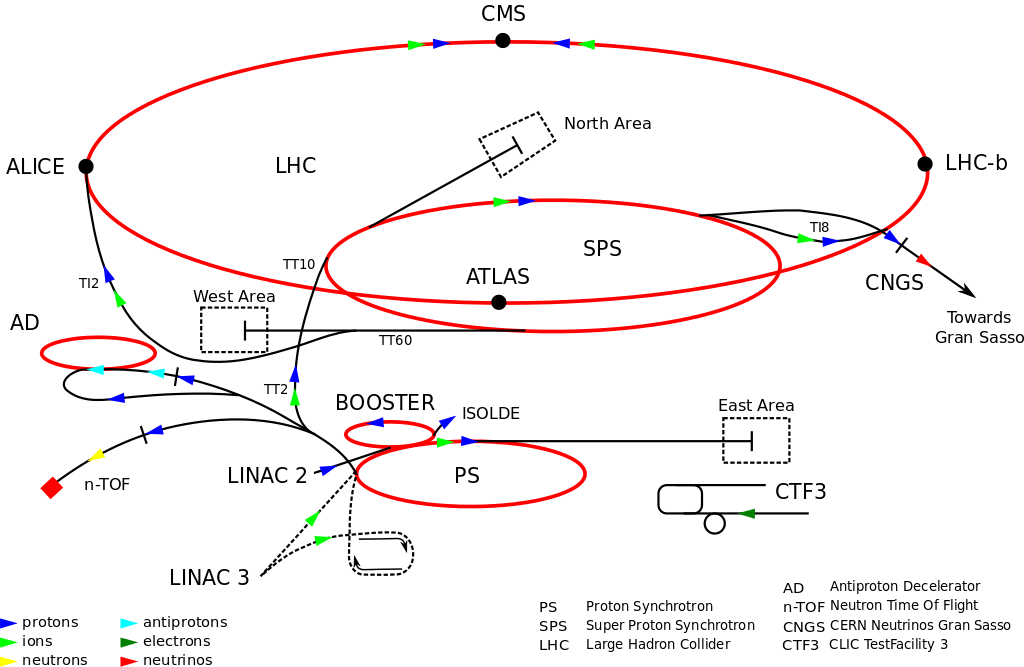
\includegraphics[width=.90\linewidth]{figures/lhc/Cern-accelerator-complex.png}
\caption{The pre-accelerators of the \ac{LHC}.}
\label{fig:preacc}
\end{figure}
\end{centering}

The chain begins with when hydrogen gas is stripped of its electrons and injected in short pulses into Linac2, a linear accelerator which uses \ac{RF} cavities, which use alternating positive and negative electric fields to simultaneously push and pull particles forward through the accelerator. This \ac{RF} behavoir keeps the bunches of protons resulting from the original pulses separated, beginning the formation of the bunch structure used for collisions. Quadropole magnets along the accelerator keep the beam focused. By the end of the accelerator, protons have reached 50 \mev. 

The proton beam is then injected into the \ac{PSB}, the first circular accelerator in the pre-accelerator chain. It increases its magnetic field as the protons increase in speed, ultimately accelerating them to 1.4 \gev. 

At this point the proton moves on to the \ac{PS}, a 600 m long circular accelerator that consists of 277 electromagnets that accelerate the protons up to 25 \gev, and 100 additional dipole magnets to bend the beam. 

The last accelerator before injection into the \ac{LHC} is the \ac{SPS}, a 7 km long ring which, long before the \ac{LHC} tunnel was built, was responsible for the discover of the $W$ and $Z$ bosons. The \ac{SPS} accelerates particles up to 450 \gev~before they are launched into the \ac{LHC}. 

Proton bunches are structured for ease of acceleration, with distinct features resulting from each of the pre-accelerators. The \ac{PS} produces 72 bunches separated by 25 ns, which are injected into the \ac{SPS}, as seen in \autoref{fig:bunches}. However, as the magnetic field directing these protons out of the \ac{PS} loop is turned on, there must be a gap in the bunch structure. Without this gap, called the injection kicker rise time, the changing magnetic field would direct particles out of the accelerator and produce high amounts of unsafe radiation around the \ac{PS}. A similar gap in bunch structure is required for the injection from the \ac{SPS} to the \ac{LHC}. The injection process is repeated until the \ac{LHC} is completely filled with around 2000 bunches, which takes about three minutes.

\begin{centering}
\begin{figure}[!hbt]
\myfloatalign
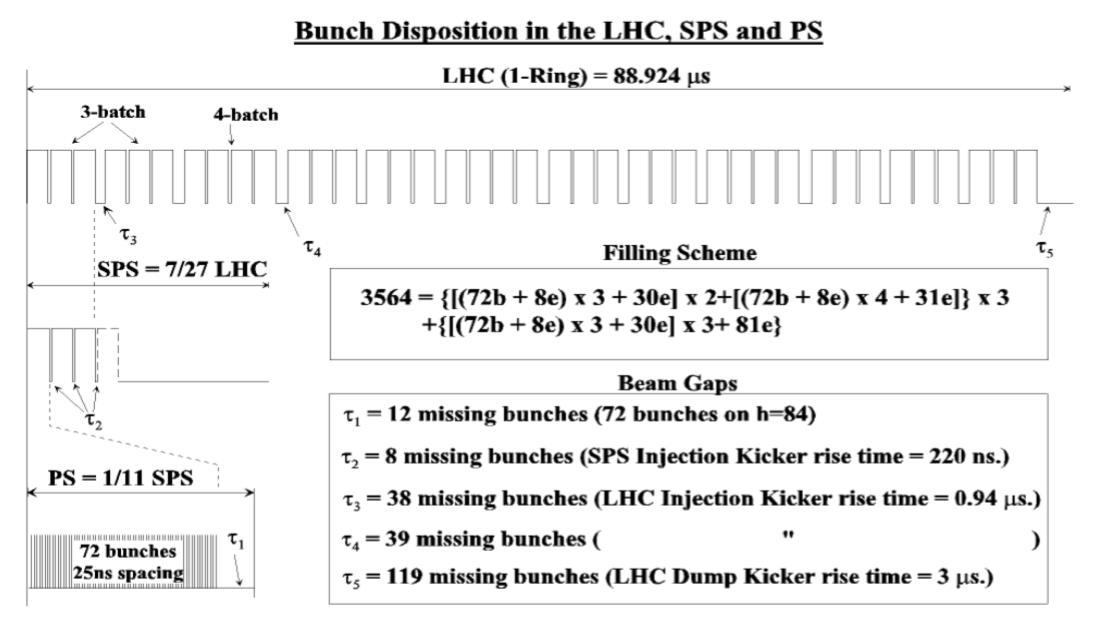
\includegraphics[width=.90\linewidth]{figures/lhc/bunch_structure.png}
\caption{Bunch structure in the \ac{PS}, \ac{SPS}, and \ac{LHC}.}
\label{fig:bunches}
\end{figure}
\end{centering}

\section{Operation of the Large Hadron Collider}

The \ac{LHC} consists of eight straight sections each connected by an arc. In each straigh section, \ac{RF} cavities accelerate protons, ultimately bringing them up to 6.5 \gev. Between these straight sections, 8.4 T dipole magnets bend the beams to maintain the approximately circular path. However, because the \ac{LHC} is a proton-proton collider as opposed to a proton-antiproton collider, the two counter-rotating beams must be housed in separate rings and be accelerated separately. To achieve this, twin-bore superconduncting magnets, one example of which can be seen in \autoref{fig:magnet}, surround the two rings and accelerate them both. Quadropole magnets are used at the four collision points to focus the beams, which cross at an interaction point at the center of a detector. In total there are 1232  main dipole magnets over 5000 additional magnets, which are all are superconducting and kept below their critical temperatures by liquid helium cooling. 

\begin{centering}
\begin{figure}[!hbt]
\myfloatalign
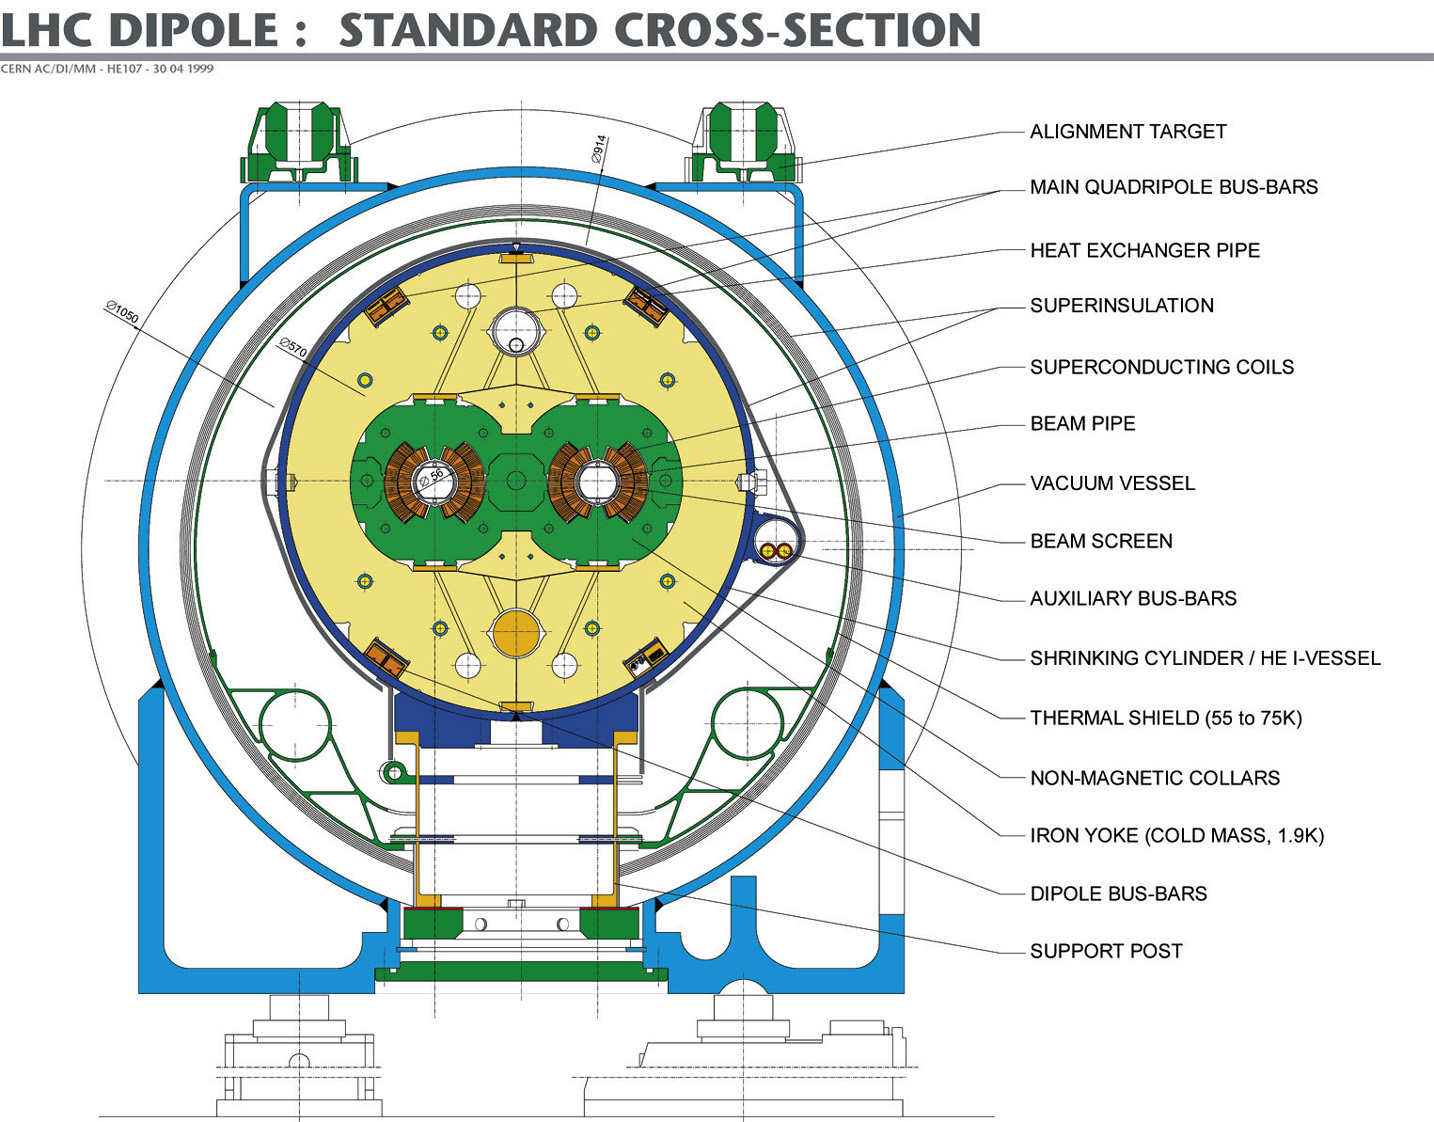
\includegraphics[width=.90\linewidth]{figures/lhc/magnet.jpg}
\caption{Cross-section of a cryodipole magnet in the \ac{LHC}.}
\label{fig:magnet}
\end{figure}
\end{centering}

When first injected into the \ac{LHC}, the protons must be accelerated over many turns through the machine, with the magentic field from the dipoles increasing with each pass to apply more force with which to bend the beam. Once the protons have reached a maximum energy, a process called ``squeezing'' occurs, in which the the total transverse area of the beam is reduced and bunches are elongated slightly. The shape produced by this process determines the ``beam spot'' for the ATLAS detector, the measurement of the area in which collisions occur within the detector. As shown in \autoref{fig:beam_spot}, the collisions all occur very close together in the $x-y$ plane, but have a long spread in the $z$ direction\footnote{The coordinate system used here is discussed in \autoref{sec:coords}.}.

\begin{centering}
\begin{figure}[!hbt]
\myfloatalign
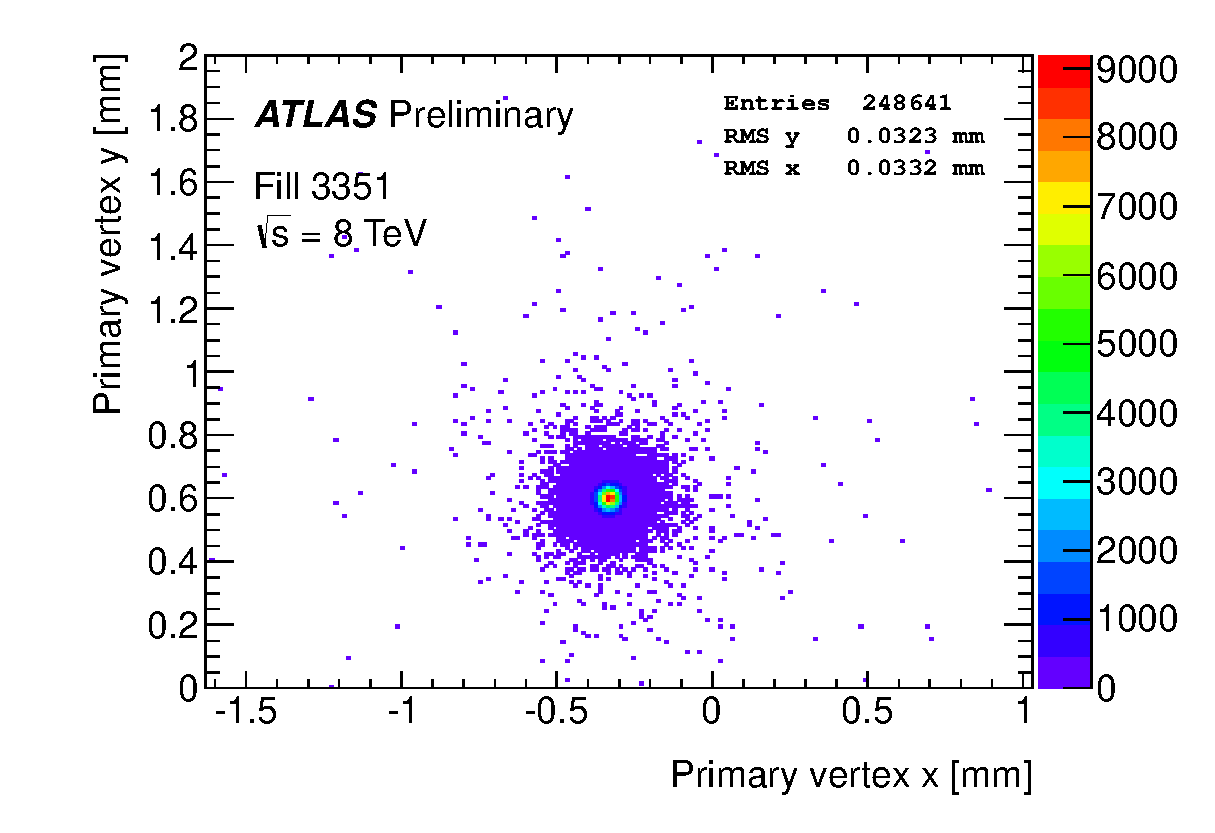
\includegraphics[width=.45\linewidth]{figures/lhc/beamspot-run215456-vtx-yx.eps}
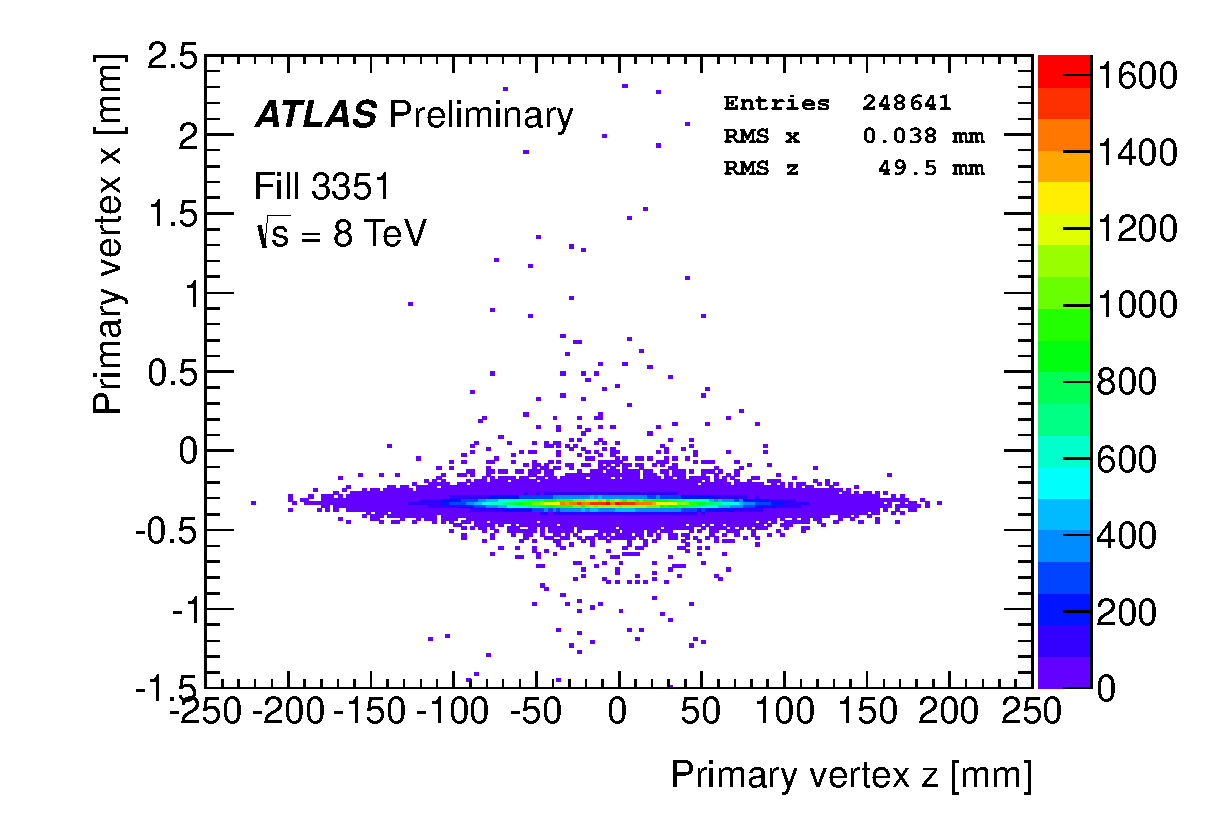
\includegraphics[width=.45\linewidth]{figures/lhc/beamspot-run215456-vtx-xz.eps}
\caption{Beam spot in the ATLAS detector for one run in 2015. Distributions show only the highest \pt vertex per event. Left is the $x-y$ distribution of vertices, while the right plot shows the $x-z$ distribution.}
\label{fig:beam_spot}
\end{figure}
\end{centering}

Once the beams are at a stable energy and have been squeezed, the \ac{LHC} indicates that it is physics-ready to the experiments around the ring, and, after some additional checks by each experiment, data-taking can begin. As collisons occur, the beam is depleted, and when it is sufficiently depleted to require a new fill, or if any instability occurs, the beam is dumped into a cavern filled with steel and concrete, which absorbs the energy. 

\section{Luminosity}

The goal of the collisions provided by the \ac{LHC} is to produce \ac{SM} and \ac{BSM} particles, which can be observed by the detectors. How frequently a given process could occur was a crucial consideration in its design. The number of events of a given type is given by

\begin{equation}
N_{event} = L\sigma_{event}
\end{equation}

where $L$ is the luminosity delivered by the \ac{LHC} and $\sigma_{event}$ is the cross-section of the process in question. These cross-sections vary over many orders of magnitude for different processes, as shown in \autoref{fig:cross_sections}, a plot of many different \ac{SM} cross-sections. As a consequence, a very large amount of luminosity is required to produce the more rare events, and to have enough statistical power to differentiate them from other much more common events.   

\begin{centering}
\begin{figure}[!hbt]
\myfloatalign
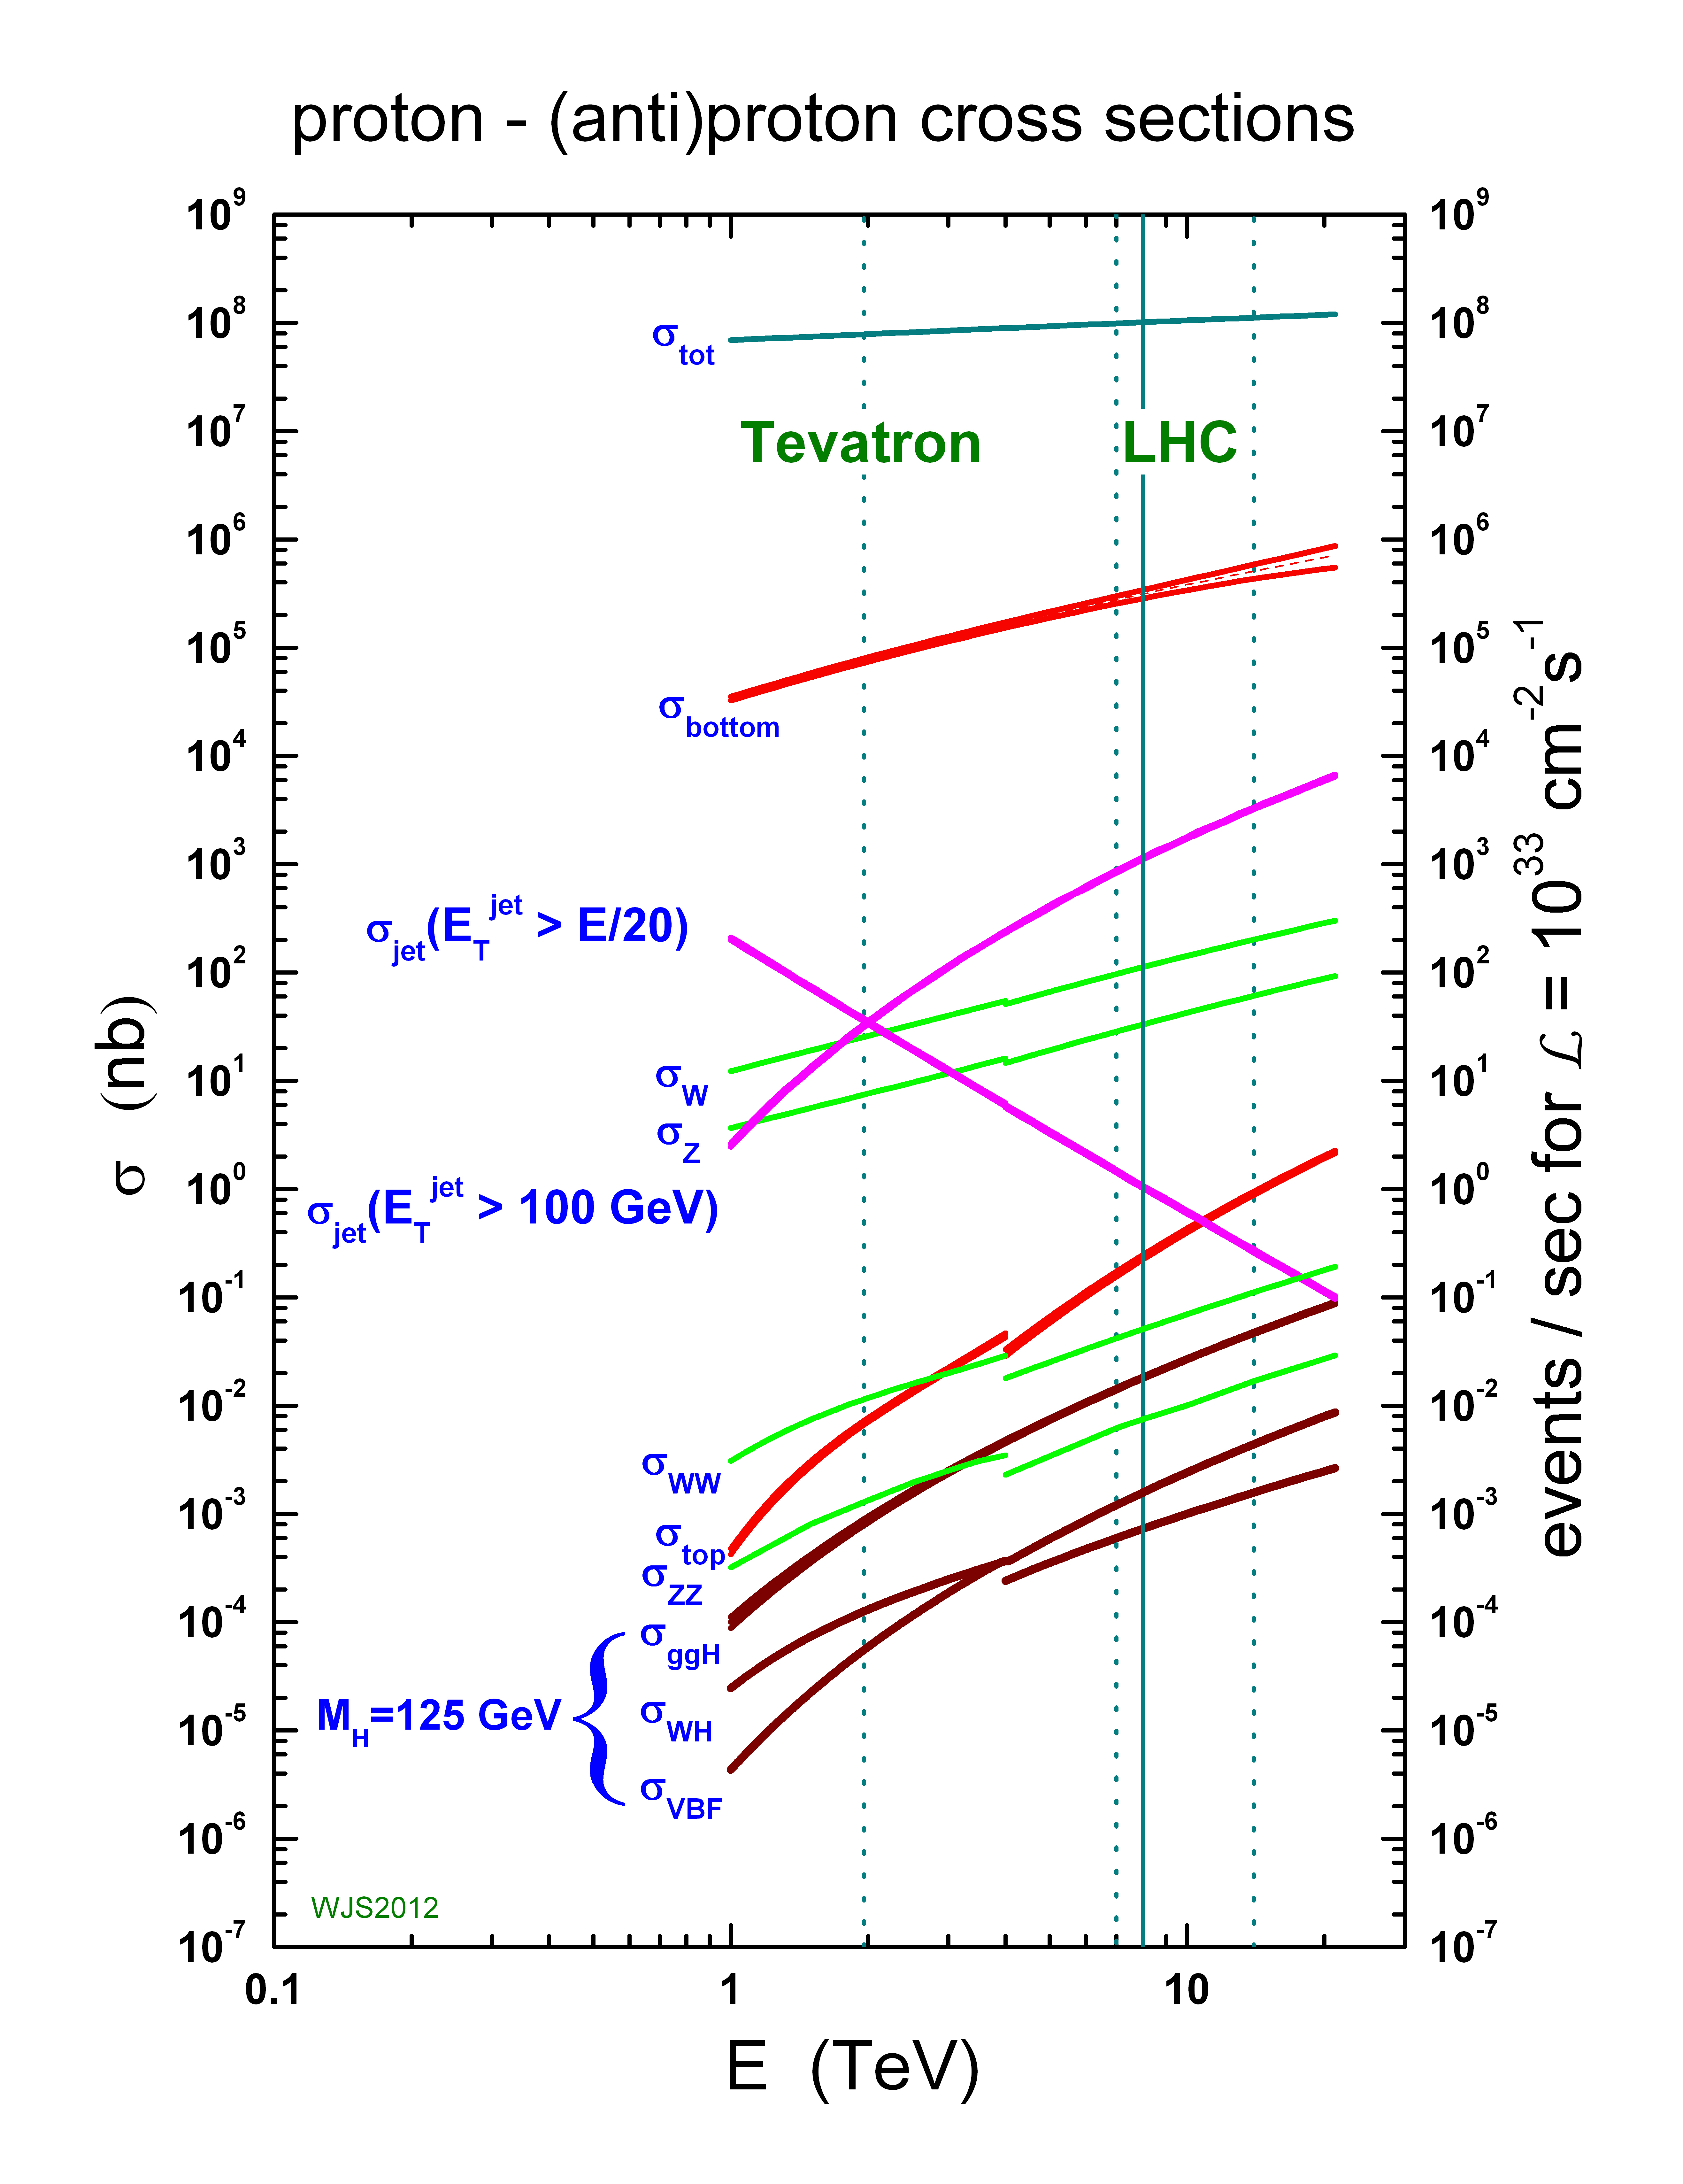
\includegraphics[width=.60\linewidth]{figures/lhc/crosssections2013.jpg}
\caption{Cross-sections for many \ac{SM} processes at the Tevatron and \ac{LHC} \cite{crosssections}.}
\label{fig:cross_sections}
\end{figure}
\end{centering}

The instantaneous luminosity at the \ac{LHC} is given by

\begin{equation}
L = \frac{ N^2_b n_b f_{rev} \gamma_r }{ 4\pi \epsilon_n \beta* } F
\end{equation}

where $N_b$ is the number of protons per bunch ($\sim10^{11}$), $n_b$ is the number of bunches in each beam ($\sim10^3$), $f_{rev}$ is the number of times per second that the beam travels around the ring, $\gamma_r$ is the relativistic gamma factor, $\epsilon_n$ is the normalized transverse beam emittance, and $\beta*$ is the $\beta$-function at the collision point, which describes the transverse displacement of particles in the beam. $F$ gives the reduction factor due to the geometry of the beam crossings, and is given by

\begin{equation}
F = (1+ (\frac{\theta_c \sigma_z}{2\sigma*})^2)^{-1/2}
\end{equation}

where $\theta_c$ is the crossing angle of the beams, $\sigma_z$ is the RMS of the bunch length in the $z$ direction, and $\sigma*$ is the same in the transverse direction.

As the proton beams circulate and collide, $N_b$ decreases, producing a falling instantaneous luminosity, as seen a Run 1 example in \autoref{fig:instlumi}. In Run 2, peak instantaneous luminosity was brought up to $10^{34}$ cm$^{-2}$s$^{-1}$. This high instantaneous luminosity and consistent running resulted in much faster data collection than in Run 1, which is depicted in \autoref{fig:lumi_vs_year}. 

\begin{centering}
\begin{figure}[!hbt]
\myfloatalign
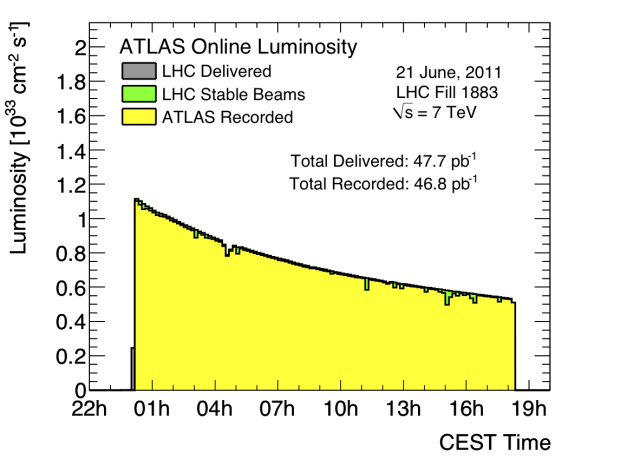
\includegraphics[width=.90\linewidth]{figures/lhc/lumi1883.jpg}
\caption{Instantaneous luminosity of one fill of 7 \tev data in 2011.}
\label{fig:instlumi}
\end{figure}
\end{centering}

\begin{centering}
\begin{figure}[!hbt]
\myfloatalign
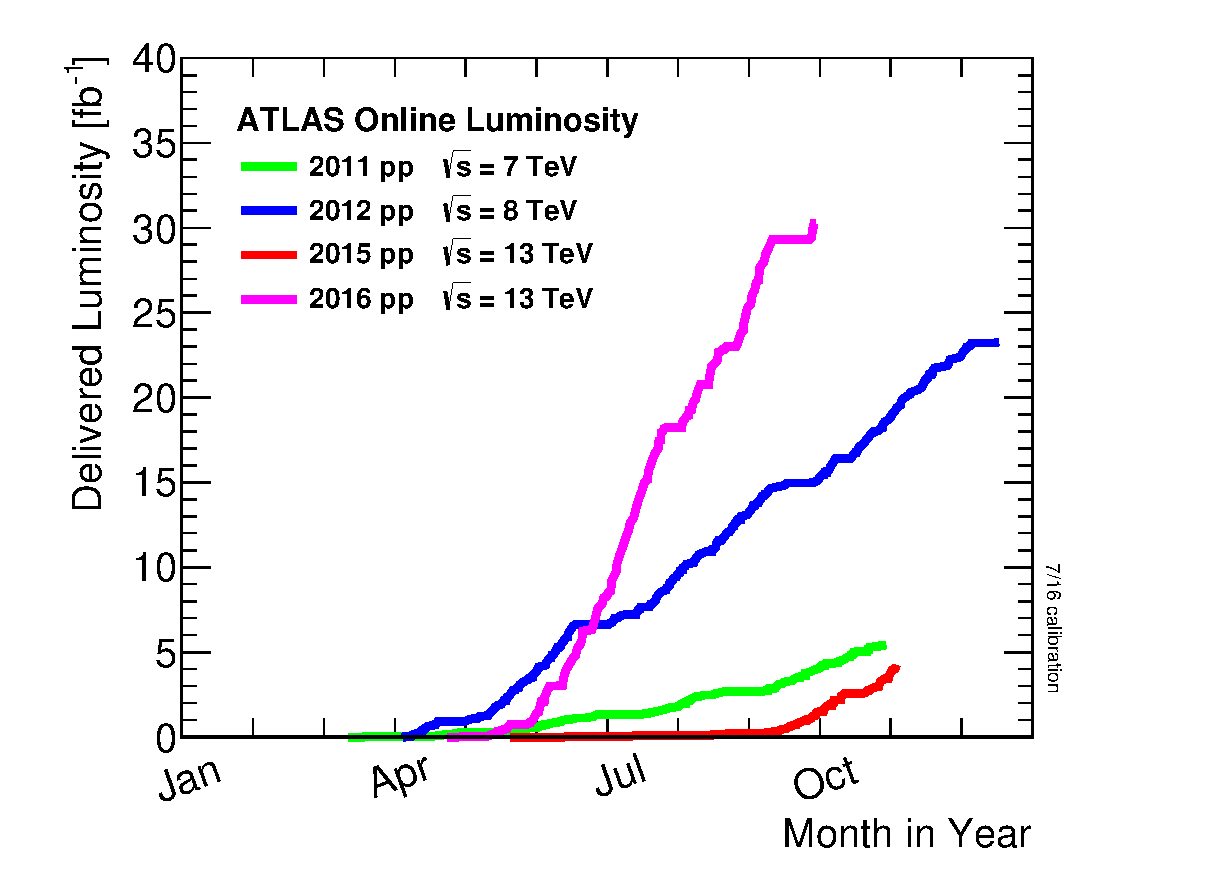
\includegraphics[width=.90\linewidth]{figures/lhc/intlumivsyear.eps}
\caption{ATLAS luminosity for Run 1 and Run 2, as of September 2016.}
\label{fig:lumi_vs_year}
\end{figure} 
\end{centering}

\section{Pile-up in proton-proton Collisions}
\label{sec:pileup}

One consequence of the high instantaneous luminosity is ``pile-up'', or multiple simultaneously interactions. Because each bunch has on order 100 billion protons, it is very likely that multiple protons will collide in the same bunch crossing. In fact, the average number of simultaneous interactions in 13 \tev data, shown in \autoref{fig:ninteractions}, is about twenty. 

\begin{centering}
\begin{figure}[!hbt]
\myfloatalign
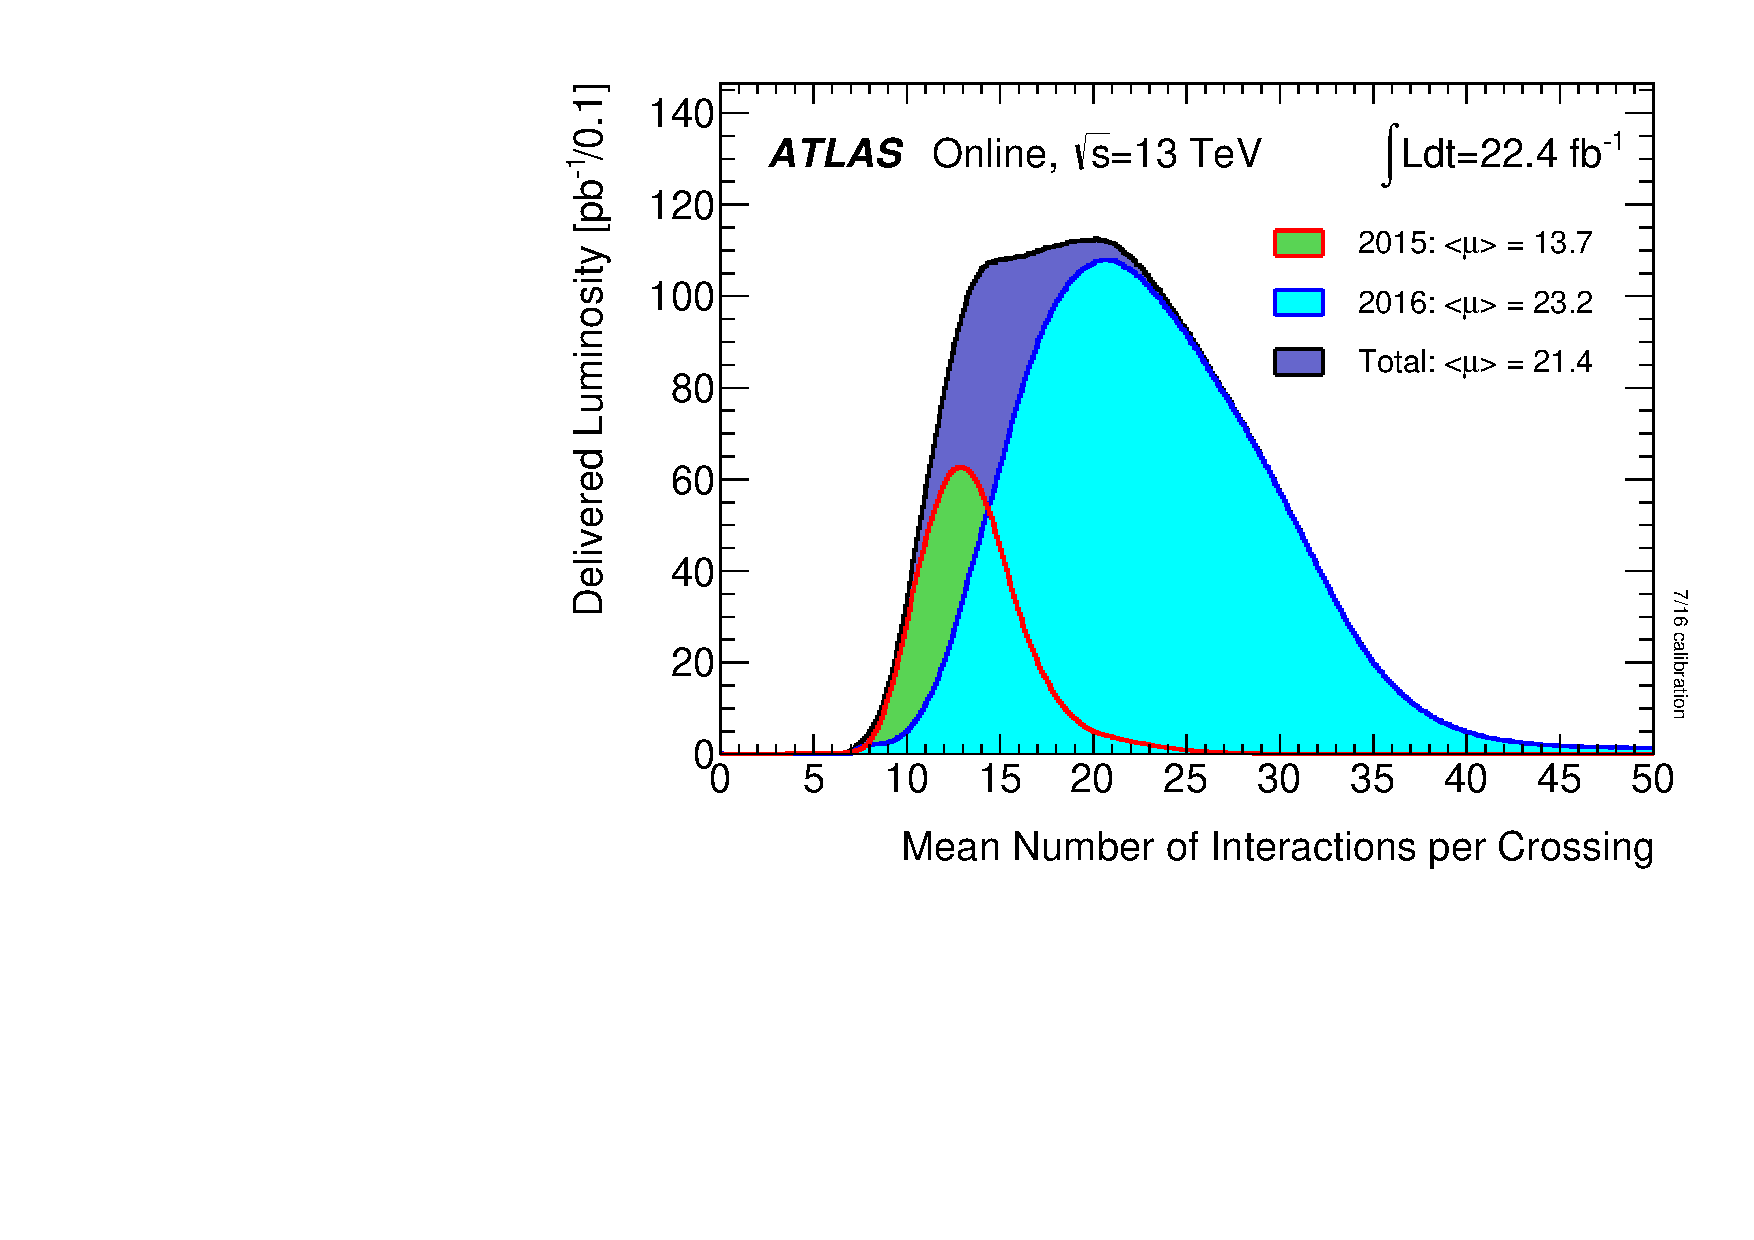
\includegraphics[width=.85\linewidth]{figures/atlas/mu_2015_2016_ICHEP.pdf}
\caption{Average number of interactions per crossing shown for 2015 and 2016 separately, as well as the sum of the two years.}
\label{fig:ninteractions}
\end{figure}
\end{centering}

Pile-up can be a difficult challenge for the ATLAS collaboration because it typically results in additional jets in an event, and can increase \ac{SM} backgrounds for analyses seeking to identify events with jets. It can also add to the overall hadronic energy of an event, and that energy can be mis-assigned to other objects. Fortunately, it is typically possible to resolve the different vertices that each proton-proton collision makes, and so pile-up jets can be identified and rejected. 


